% Don't modify this section unless you know what you're doing!
\documentclass[letterpaper,12pt]{article}
\usepackage{float}
\usepackage[spanish]{babel}
\selectlanguage{spanish}
\usepackage[utf8]{inputenc}
\usepackage{tabularx} % extra features for tabular environment
\usepackage{amsmath}  % improve math presentation
\usepackage{graphicx, wrapfig, subcaption, setspace, booktabs}
\usepackage{graphicx} % takes care of graphic including machinery

\usepackage[margin=1in,letterpaper]{geometry} % decreases margins
\usepackage{cite} % takes care of citations
\usepackage[final]{hyperref} % adds hyper links inside the generated pdf file
\usepackage{amsmath}
\usepackage{amssymb}
\usepackage{enumerate}
\usepackage{url}
\hypersetup{
	colorlinks=true,       % false: boxed links; true: colored links
	linkcolor=blue,        % color of internal links
	citecolor=blue,        % color of links to bibliography
	filecolor=magenta,     % color of file links
	urlcolor=blue         
}
%++++++++++++++++++++++++++++++++++++++++
\documentclass{article}
\usepackage[utf8]{inputenc}

\title{Actividad 10}
\author{Daniela Olmos Velderrain}
\date{16 de mayo del 2019}

\begin{document}

\maketitle

\section{Introducción}
 En esta actividad se resolvió numéricamente la ecuación de Duffing, la cual es una ecuación diferencial no lineal de segundo orden. Mediante la función \emph{ode} de \emph{SciPy} se empleó el método de Runge-Kutta de cuarto orden para su resolución.\\\\
 Se generaron gráficas para mostrar el comportamiento de las soluciones al variar un parámetro de la ecuación, así como una gráfica donde se resuelve el sistema tomando en cuenta su evolución, y así intentar determinar si dicho sistema presenta el fenómeno de histéresis.
 
           
\section{Desarrollo}
            
\subsection{Marco teórico}
\subsubsection{Ecuación de Duffing}
La ecuación de Duffing describe un oscilador no lineal de segundo orden. Esta ecuación modela un resorte con un rozamiento proporcional a la velocidad, el cual está sometido a la acción de una fuerza periódica. La ecuación está dada por:

\[\Ddot{x} + \delta \Dot{x} + \alpha x + \beta x^{3} = \gamma cos( \omega t)\]

Los parámetros en la ecuación son:
\begin{itemize}
    \item $\delta$ := Factor de amortiguamiento 
    \item $\alpha$ := Rigidez 
    \item $\beta$ := No linealidad 
    \item $\gamma$ := Amplitud de la fuerza impulsora
    \item $\omega$ := Frecuencia angular de la fuerza impulsora 
\end{itemize}


\subsubsection{Histéresis}
La histéresis es un fenómeno debido al cual un material presenta una evolución que no solo depende de la causa que lo provoca, sino también de cada uno de sus estados anteriores.\\\\\
La histéresis se puede presentar, por ejemplo, en el momento magnético de un imán, el cual va a depender de la forma en que evolucione el campo magnético.\\
Como este hay otros ejemplos de histéresis que pueden encontrarse en física, química, ingeniería y otras áreas de la ciencia.\\ 
En los sistemas naturales es comunmente asociada con cambios termodinámicos irreversibles, tales como transiciones de fase y con fricción interna.
\\\\
Los sistemas con histéresis son no lineales y matemáticamente difíciles de modelar.



\subsection{Metodología}
Para poder resolver la ecuación diferencial de Duffing mediante $ode$, necesitamos separarla en dos ecuaciones de primer orden mediante un cambio de variable:

\[\Dot{x} = y\]
\[\Dot{y}= - \delta y - \alpha x - \beta x^{3} + \gamma cos( \omega t)\]

Definimos estas ecuaciones en una función, donde los parámetros de inegración son $x$ y $y$.\\

Para realizar la primera gráfica fue necesario resolver las ecuaciones para varios valores de $\beta$, por lo cual se creó un arreglo de dichos valores y mediante un loop se graficaron cada uno de los resultados.\\

Las condiciones iniciales empleadas para la primera gráfica fueron las siguientes:  

\begin{table}[H]
     &  \\
     & 
\label{tabla:1}
\centering
\caption{Parámetros y condiciones iniciales.}
\begin{tabular*}{10 cm}{|l|l@{\extracolsep{\fill}}r|}
\hline
Parámetro                       &    Valores                &\\
\hline
\delta                          &         0.1               &\\
\alpha                          &         1.0               &\\
\beta                           &  -0.003, 0.0, 0.01, 0.04  &\\
\gamma                          &         1.0               &\\
\omega                          &      0.0 a 2.5            &\\
Ancho de paso                   &         0.1               &\\
x                               &         1.0               &\\
y                               &         0.0               &\\
\hline
\end{tabular*}
\end{table}

Luego de obtener las soluciones, se almacenaron en arreglos la amplitud máxima y el valor correspondiente de $\omega$.\\\\

En el caso de la segunda gráfica fue necesario resolver la ecuación diferencial para valores de $\omega$ avanzando hasta cierto valor y luego retrocediendo hasta el punto de inicio.\\\\

Para esto se guardó la información en dos gráficas, una gráfica de \emph{ida} y otra de \emph{vuelta} (para lograr esto se hizo que $\omega$ retrocediera en el contador). Las condiciones iniciales fueron las mismas que en la primera gráfica (con $\beta$=0.04).\\\\

Al resolver la ecuación diferencial en este caso se empleó en cada iteración la condición inicial de la iteración anterior.

\section{Resultados}
La gráfica obtenida para los diferentes valores de $\beta$ es la siguiente:

\begin{figure}[H]
\centering
\fbox{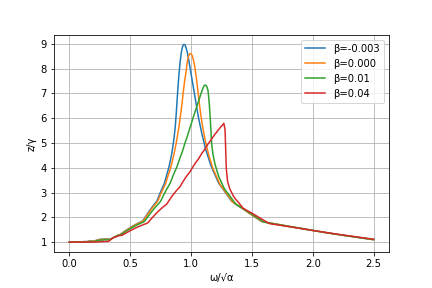
\includegraphics[width=0.5\linewidth]{graf1.png}}
\caption{Respuesta de frecuencia basada en la ecuación de Duffing.}
\label{fig:esquema2}
\end{figure}

En las primera gráfica podemos observar que las pendientes y el valor máximo de la amplitud cambian dependiendo del valor de $\beta$. Para el valor negativo de $\beta$ la gráfica está inclinada hacia la izquierda y se registra la amplitud más grande para los valores de $\beta$ probados; en cambio, para valores negativos las amplitudes son cada vez menores y la pendiente, antes de que la gráfica alcance su valor máximo, es positiva y cada vez menos pronunciada. \\\\

En la segunda gráfica observamos un comportamiento peculiar:

\begin{figure}[H]
\centering
\fbox{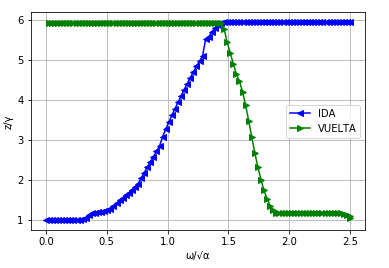
\includegraphics[width=0.5\linewidth]{graf22.png}}
\caption{Histéresis en el oscilador de Duffing.}
\label{fig:esquema2}
\end{figure}

Aquí podemos observar que la gráfica comienza con un comportamiento normal, tanto de ida como de regreso, pero una vez alcanzando su valor máximo ambas gráficas son constantes.


\section{Conclusiones}
  El oscilador de Duffing describe las oscilaciones de una masa unida a un resorte no lineal y un amortiguador lineal.
  Aquí la fuerza restauradora dada por el resorte no lineal es $\alpha x+\beta x^{3}$.
\\\\
Cuando $\alpha>0$ y $\beta>0$ el resorte es llamado \emph{resorte de endurecimiento}; cuando $\beta<0$ es llamado \emph{resorte de reblandecimiento}. Por otra parte, si $\beta=0$, el oscilador se comporta como un oscilador simple amortiguado e impulsado. 
\\\\
Este comportamiento es el observado en la respuesta de frecuencia de la primera gráfica, lo cual puede explicar por qué conforme incrementa el valor de $\beta$ las oscilaciones parecen ser de menor amplitud.
\\\\
En la segunda gráfica, donde se toma en cuenta la evolución de las condiciones iniciales, el oscilador parece llegar alcanzar un valor crítico para el cual los valores son constantes. Esto ocurre una vez que se alcanza la amplitud máxima en cierto valor de $\omega$, concidiendo cuando se avanza hacia delante y hacia atrás.\\\\

Tal parece que el algoritmo no puede recuperarse pasando este punto, por lo cual, sin importar que cambien los valores de $\omega$, la respuesta de frecuencia permanece constante. Esto podría ocurrir debido a que el oscilador se detiene luego de alcanzar una velocidad crítica, para la cual la fuerza de amortiguamiento (proporcional a $\Dot{x}$) es suficiente para detener las fuerzas restauradoras en el resorte, mostrando así solo la amplitud máxima obtenida en la iteración anterior. 



\section*{Bibliografía}
\begin{itemize}
\item \\Histéresis. Recuperado el 27 de mayo de 2019 desde \\https://es.thefreedictionary.com/hist\%C3\%A9resis
\\

\item \\Histéresis. Recuperado el 27 de mayo de 2019 desde \\https://en.wikipedia.org/wiki/Hysteresis
\\

\item \\Duffing Equation. Recuperado el 27 de mayo de 2019 desde \\https://en.wikipedia.org/wiki/Duffing\_equation
\\


\end{itemize}



\end{document}
